\documentclass[conference,a4paper]{IEEEtran} %enable this for camera ready (by ABJ)
% \documentclass[conference,peerreview,a4paper]{IEEEtran} %enable this for peer review (by ABJ)

\IEEEoverridecommandlockouts

% IEEEtran's built-in a4paper margins fall short of EDAS PDFExpress's required
% margins (1.57cm side, 1.9cm top, 2.9cm bottom). Override explicitly with
% headroom so the camera-ready PDF passes the check.
\usepackage[a4paper,left=1.85cm,right=1.85cm,top=2.1cm,bottom=3.2cm]{geometry}

% ---- packages ----
\usepackage{cite}
\usepackage{amsmath,amssymb,amsfonts}
\usepackage{algorithmic}
\usepackage{graphicx}
\usepackage{textcomp}
\usepackage{xcolor}
\usepackage{listings}
\usepackage{booktabs}
\usepackage{array}
\usepackage{url} 


\def\BibTeX{{\rm B\kern-.05em{\sc i\kern-.025em b}\kern-.08em
    T\kern-.1667em\lower.7ex\hbox{E}\kern-.125emX}}

% --- Advanced Spacing Optimizations ---
\usepackage{microtype}
\setlength{\textfloatsep}{6pt plus 1pt minus 1pt}
\setlength{\intextsep}{6pt plus 1pt minus 1pt}
\setlength{\floatsep}{5pt plus 1pt minus 1pt}
\setlength{\abovedisplayskip}{3pt}
\setlength{\belowdisplayskip}{3pt}
\setlength{\abovedisplayshortskip}{2pt}
\setlength{\belowdisplayshortskip}{2pt}

\AtBeginDocument{\def\IEEEkeywordsname{Keywords}}

\begin{document}

\title{A Comprehensive Parasitic-Aware Post-Layout Design and Verification Methodology for a 6.5-GHz Ultra-Low-Power Ring Oscillator in 65-nm CMOS}

\author{\IEEEauthorblockN{Abidul Qohar}
\IEEEauthorblockA{\textit{Department of Electrical Engineering} \\
\textit{and Information Technology} \\
\textit{Faculty of Engineering}\\
\textit{Universitas Gadjah Mada} \\
Yogyakarta, Indonesia \\
abidulqohar@mail.ugm.ac.id}
\and
\IEEEauthorblockN{Prapto Nugroho}
\IEEEauthorblockA{\textit{Department of Electrical Engineering} \\
\textit{and Information Technology} \\
\textit{Faculty of Engineering}\\
\textit{Universitas Gadjah Mada} \\
Yogyakarta, Indonesia \\
tatok@ugm.ac.id \\
\textit{*corresponding author}
}
\and
\IEEEauthorblockN{Dzuhri Radityo Utomo}
\IEEEauthorblockA{\textit{Department of Electrical Engineering} \\
\textit{and Information Technology} \\
\textit{Faculty of Engineering}\\
\textit{Universitas Gadjah Mada} \\
Yogyakarta, Indonesia \\
dzuhri.r.u@ugm.ac.id}
\and[\\\mbox{}\hfill]
\IEEEauthorblockN{Agus Bejo}
\IEEEauthorblockA{\textit{Department of Electrical Engineering} \\
\textit{and Information Technology} \\
\textit{Faculty of Engineering}\\
\textit{Universitas Gadjah Mada} \\
Yogyakarta, Indonesia \\
agusbj@ugm.ac.id}
\and[\hspace{3em}]
\IEEEauthorblockN{Eka Firmansyah}
\IEEEauthorblockA{\textit{Department of Electrical Engineering} \\
\textit{and Information Technology} \\
\textit{Faculty of Engineering}\\
\textit{Universitas Gadjah Mada} \\
Yogyakarta, Indonesia \\
eka.firmansyah@ugm.ac.id}
}
\maketitle %enable this for camera ready (by ABJ)
% \IEEEpeerreviewmaketitle %enable this for peer reveiw (by ABJ)

\begin{abstract}
This paper reports the physical implementation and parasitic-aware post-layout
characterization of a low-power three-stage CMOS ring oscillator implemented in
a 65-nm Low-Power (LP) CMOS process. Operating from a 1.0-V supply, the
oscillator is physically implemented using custom layout techniques with a
compact active area of $73.96~\mu\text{m}^2$. Following successful design rule
checking (DRC), Layout Versus Schematic (LVS) verification, and detailed
standard parasitic format (DSPF) extraction, post-layout Periodic Steady State
(PSS) and periodic noise (\texttt{pnoise}) analyses are performed to
characterize the oscillator under realistic conditions. The extracted design
achieves a stable oscillation frequency of 6.50~GHz while consuming only
$286.3~\mu$W from a 1.0-V supply. The simulated single-sideband phase noise is
$-77.6$~dBc/Hz at a 1-MHz offset, corresponding to a figure of merit (FoM) of
$-159.3$~dBc/Hz. The comparison between schematic and post-layout simulations
highlights the significant influence of distributed interconnect parasitics on
oscillator performance, emphasizing the importance of parasitic-aware physical
verification in nanoscale CMOS circuits. The results provide a concrete
reference point for the parasitic budget that must be anticipated when designing
low-power multi-gigahertz oscillators in nanoscale CMOS.
\end{abstract}

\begin{IEEEkeywords}
ring oscillator, CMOS, post-layout verification, parasitic extraction, DSPF, phase noise, low-power design
\end{IEEEkeywords}

\section{Introduction}
Oscillators are essential building blocks in modern integrated circuits and are
widely used in phase-locked loops (PLLs), clock-and-data recovery (CDR)
circuits, and other timing systems~\cite{maneatis_dll}. Among various oscillator
topologies, ring oscillators are attractive because they occupy a small silicon
area, do not require inductors, and can be readily implemented in standard CMOS
processes~\cite{razavi_analog, lee_cmos}. In particular, the three-stage ring
oscillator offers a simple structure and naturally provides multiple phase
outputs, making it suitable for many high-speed
applications~\cite{maneatis_coupled, nugroho_ring}.

As CMOS technology scales into the nanometer regime, however, maintaining the
accuracy of circuit performance prediction becomes increasingly challenging.
During the early design stage, circuit performance is commonly evaluated using
schematic-level simulations. While this approach is useful for initial design
exploration, it does not account for parasitic elements introduced during
physical implementation. At multi-gigahertz frequencies, interconnect
resistances and capacitances in the back-end-of-line (BEOL) layers can no longer
be neglected. These parasitic components increase signal propagation delay and
may cause the actual oscillation frequency to deviate from the intended design
value~\cite{hajimiri_ring}.

For this reason, post-layout verification plays an important role in
high-frequency circuit design. Although many studies have reported the
performance of CMOS ring oscillators, most discussions focus on transistor-level
simulations, while the influence of layout parasitics is often treated only
briefly. As technology nodes continue to shrink, understanding the difference
between schematic and post-layout performance becomes increasingly important for
obtaining reliable circuit behavior.

In this work, a low-power three-stage ring oscillator is implemented in a 65-nm
Low-Power (LP) CMOS process and evaluated using a complete post-layout design
flow. After layout generation, the circuit is verified through design rule
checking (DRC) and layout-versus-schematic (LVS) procedures, followed by RC
parasitic extraction in Detailed Standard Parasitic Format (DSPF). The extracted
netlist is then analyzed using periodic steady-state (PSS) and periodic noise
(\texttt{pnoise}) simulations to characterize the oscillator under realistic
operating conditions.

The main contributions of this paper are summarized as follows:
\begin{itemize}
\item A node-resolved quantification of BEOL parasitic loading in a 65-nm
multi-gigahertz ring oscillator, in which per-net extracted capacitances are
reported alongside the resulting 41.7\% frequency reduction and 71.2\%
stage-delay increase.
\item A comparison between schematic-level and extracted-netlist simulations to
evaluate the effect of BEOL interconnect parasitics on oscillation frequency and
propagation delay.
\item Post-layout characterization of a compact 6.5-GHz ring oscillator with a
power consumption of $286.3~\mu$W, including phase-noise and figure-of-merit
analysis.
\end{itemize}

\section{Ring Oscillator Operation and Design Methodology}

\subsection{Topology Selection}

A ring oscillator was selected for this study. Compared with LC oscillators,
which offer superior phase noise but require a large die area and an on-chip
inductor, ring oscillators occupy considerably less area, maintain a relatively
constant voltage swing, operate at low supply voltages, and can be realized in
any standard CMOS process without additional passive
components~\cite{razavi_analog, lee_cmos}. These properties suit the
$73.96~\mu\text{m}^2$ core budget and the 1.0-V supply targeted here.

Beyond area and power, the ring oscillator has a further property that makes it
well suited to the purpose of this work: its oscillation frequency is directly
and explicitly governed by the propagation delay of its stages, as developed in
the following subsection. Any change in node capacitance therefore appears
directly as a measurable frequency shift. This makes the ring oscillator an
effective vehicle for evaluating switching speed and the influence of design and
layout parameters on propagation delay, which is the central concern of this
paper.

The three-stage configuration was adopted because it is the minimum odd stage
count that satisfies the Barkhausen criterion for a single-ended inverter ring,
and has been reported successfully in prior work~\cite{nugroho_ring}. A smaller
stage count also minimizes the total switched capacitance around the loop,
which is consistent with the low-power target.

\subsection{Oscillation Principle and Startup Condition}
The proposed oscillator consists of three cascaded CMOS inverter stages
connected in a closed loop. Each stage is formed by a PMOS--NMOS pair, and the
output of the last stage is fed back to the input of the first stage. Because the
loop contains an odd number of inversions, the circuit is able to generate a
self-sustained periodic signal.

To maintain oscillation, the loop must satisfy the Barkhausen criterion at the
oscillation frequency. This requires the total phase shift around the loop to
reach $360^{\circ}$ and the loop gain to be equal to or greater than
unity~\cite{razavi_analog}. In a three-stage ring oscillator, the inverter chain
contributes an overall phase inversion of $180^{\circ}$, while the
frequency-dependent phase shift provided by the stages contributes the remaining
$180^{\circ}$ required for sustained oscillation.

Assuming that all stages are identical, the oscillation frequency can be
related to the dominant pole frequency $\omega_p$ of each stage by
$\omega_0 = \omega_p \tan(\pi/N)$, which for $N = 3$ gives
$\omega_0 = \sqrt{3}\,\omega_p$. Although this relationship is useful
analytically, the oscillation frequency is more conveniently expressed in terms
of the propagation delay of each stage. For an $N$-stage ring oscillator, the
oscillation frequency can be approximated by

\begin{equation}\label{eq:fosc_tau}
f_{\text{osc}} = \frac{1}{2N\tau_p}
\end{equation}
where $\tau_p$ denotes the average propagation delay of one stage. Since the
propagation delay is mainly determined by the effective resistance and load
capacitance of the inverter, it can be approximated by
\begin{equation}\label{eq:tau_rc}
\tau_p \approx 0.69\,R_{\text{eq}} C_{\text{tot}}
\end{equation}
where $R_{\text{eq}}$ is the equivalent switching resistance and $C_{\text{tot}}$
is the total capacitance seen at the output node. Substituting \eqref{eq:tau_rc}
into \eqref{eq:fosc_tau} gives
\begin{equation}\label{eq:fosc_rc}
f_{\text{osc}} \approx \frac{1}{1.38\,N R_{\text{eq}} C_{\text{tot}}}
\end{equation}

In practical implementations, the total capacitance consists of both intrinsic
load capacitance and parasitic capacitance introduced during physical layout.
Therefore,
\begin{equation}\label{eq:ctot}
C_{\text{tot}} = C_L + C_{\text{par}}
\end{equation}
where $C_L$ represents the intrinsic load capacitance and $C_{\text{par}}$
denotes the parasitic capacitance associated with interconnect routing and
device layout. Consequently, the oscillation frequency can be rewritten as
\begin{equation}\label{eq:fosc_par}
f_{\text{osc}} \approx \frac{1}{1.38\,N R_{\text{eq}}\left(C_L + C_{\text{par}}\right)}
\end{equation}

Equation~\eqref{eq:fosc_par} shows that additional parasitic capacitance
increases the stage delay and reduces the oscillation frequency. This effect
becomes increasingly significant at multi-gigahertz frequencies, where
interconnect parasitics can no longer be neglected. Therefore, accurate
prediction of oscillator performance requires post-layout parasitic extraction
and verification, which form the main focus of this work.

\subsection{Short-Channel Propagation Delay Model}
Although the startup condition of a ring oscillator can be explained using
small-signal analysis, its steady-state oscillation frequency is primarily
determined by the propagation delay of the inverter stages. For an $N$-stage ring
oscillator, one complete period corresponds to the time required for a signal
transition to propagate twice around the loop. Therefore,
\begin{equation}\label{eq:period}
T = \frac{1}{f_{\text{osc}}} = 2N t_d
\end{equation}
where $t_d$ denotes the average propagation delay of a single stage.


The classical long-channel estimate $t_d \approx C_{\text{node}}
V_{\text{DD}}/2I_{\text{drive}}$ becomes less accurate in 65-nm devices, where
velocity saturation and mobility degradation limit the available drain current
and the delay is instead set by the saturation current
$I_{\text{sat}} = v_{\text{sat}} C_{\text{ox}} W(V_{\text{GS}} - V_{\text{th}}
- V_{\text{dsat}})$. In either regime, however, $t_d$ remains proportional to
the effective node capacitance, which at the schematic level consists only of
intrinsic device capacitance but after physical implementation also includes
the interconnect contribution $C_{\text{par}}$ of \eqref{eq:ctot}. This effect
is examined quantitatively through post-layout extraction in the following
sections.

\subsection{Pre-Layout Performance Baseline}
Fig.~\ref{fig:schematic_capture} shows the schematic of the proposed three-stage
CMOS ring oscillator, and Table~\ref{tab:transistor_sizing} summarizes the
corresponding device dimensions. To provide a reference for evaluating the
impact of layout parasitics, the circuit was first simulated at the schematic
level using a supply voltage of $V_{\text{DD}} = 1.0$~V under typical-typical
(TT) process conditions at $27^{\circ}$C. All transistors employ a channel
length of 60~nm. The NMOS and PMOS devices are sized to $W_n = 2~\mu$m and $W_p
= 4~\mu$m, respectively, to provide balanced drive strength.

\begin{figure}[!b]
\centerline{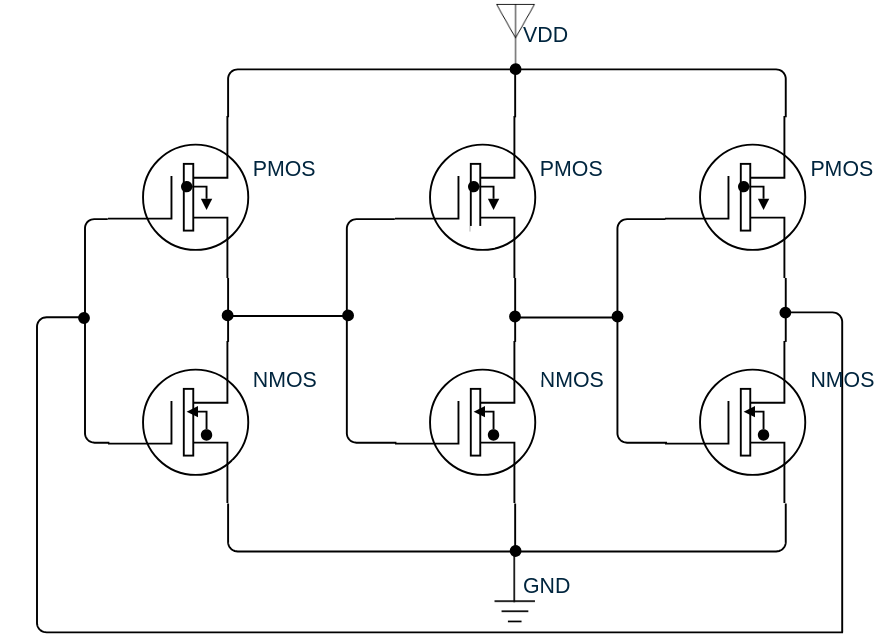
\includegraphics[width=0.40\textwidth]{sch_sd.png}}
\caption{Schematic of the verified three-stage static CMOS ring oscillator loop.}
\label{fig:schematic_capture}
\end{figure}

\begin{table}[!b]
\caption{Transistor Dimensions of the Three-Stage Ring Oscillator}
\label{tab:transistor_sizing}
\begin{center}
\begin{tabular}{cccc}
\toprule
\textbf{Device Class} & \textbf{Model} & \textbf{Width ($W$)} & \textbf{Length ($L$)} \\
\midrule
NMOS (3 devices) & \texttt{nch} & $2.0~\mu$m & 60~nm \\
PMOS (3 devices) & \texttt{pch} & $4.0~\mu$m & 60~nm \\
\bottomrule
\end{tabular}
\end{center}
\end{table}

Under these conditions, the transient simulation produces an oscillation
frequency of
\begin{equation}\label{eq:fsch}
f_{\text{osc,schematic}} = 11.15~\text{GHz}
\end{equation}
which corresponds to a period of
\begin{equation}\label{eq:tsch}
T_{\text{schematic}} = \frac{1}{f_{\text{osc,schematic}}} = 89.71~\text{ps}.
\end{equation}
Using \eqref{eq:period}, the average propagation delay of a single inverter stage
can be estimated as
\begin{equation}\label{eq:tdsch}
t_{\text{d,schematic}} = \frac{T_{\text{schematic}}}{2N} = 14.95~\text{ps}
\end{equation}
for the three-stage configuration ($N=3$). These results serve as the pre-layout
performance baseline and are later used to quantify the influence of interconnect
parasitics extracted from the physical layout.

\section{Physical Design and Custom Layout Methodology}

The physical-design and verification flow followed in this work proceeds from
schematic capture to manual layout drawing, DRC, LVS, RC parasitic extraction in
DSPF, and finally post-layout PSS and \texttt{pnoise} characterization. The
layout steps are described in this section; extraction and post-layout
simulation are described in Section~\ref{sec:pex}.

\subsection{Device Sizing and Symmetry Considerations}
The ring oscillator was implemented in a 65-nm Low-Power (LP) CMOS process. To
obtain balanced rise and fall transitions, the PMOS devices were sized twice as
wide as the NMOS devices, with $W_p = 4~\mu$m and $W_n = 2~\mu$m. This sizing
ratio compensates for the lower hole mobility of PMOS transistors and helps
maintain similar pull-up and pull-down drive strengths~\cite{razavi_rf}.

All transistors employ the minimum channel length of 60~nm to maximize switching
speed and reduce intrinsic delay~\cite{razavi_analog}. The resulting symmetric
inverter structure improves transition balance and helps minimize duty-cycle
distortion in the oscillation waveform.

\subsection{Floorplanning and Interconnect Routing}
A fully custom layout was used to implement the oscillator core, shown in
Fig.~\ref{fig:layout_core}. To simplify routing and maintain symmetry, the three
PMOS devices were placed in the upper row within a common n-well, while the
corresponding NMOS devices were arranged in the lower row. This arrangement
provides a compact structure and reduces unnecessary routing overhead.

The feedback paths between stages were routed using short interconnects primarily
in the lower metal layers. Since the oscillator operates in the multi-gigahertz
range, minimizing interconnect length is important to reduce parasitic resistance
and capacitance~\cite{razavi_rf}. The final layout occupies an area of
$8.6~\mu\text{m} \times 8.6~\mu\text{m}$, corresponding to a total core area of
$73.96~\mu\text{m}^2$.

\begin{figure}[!t]
\centerline{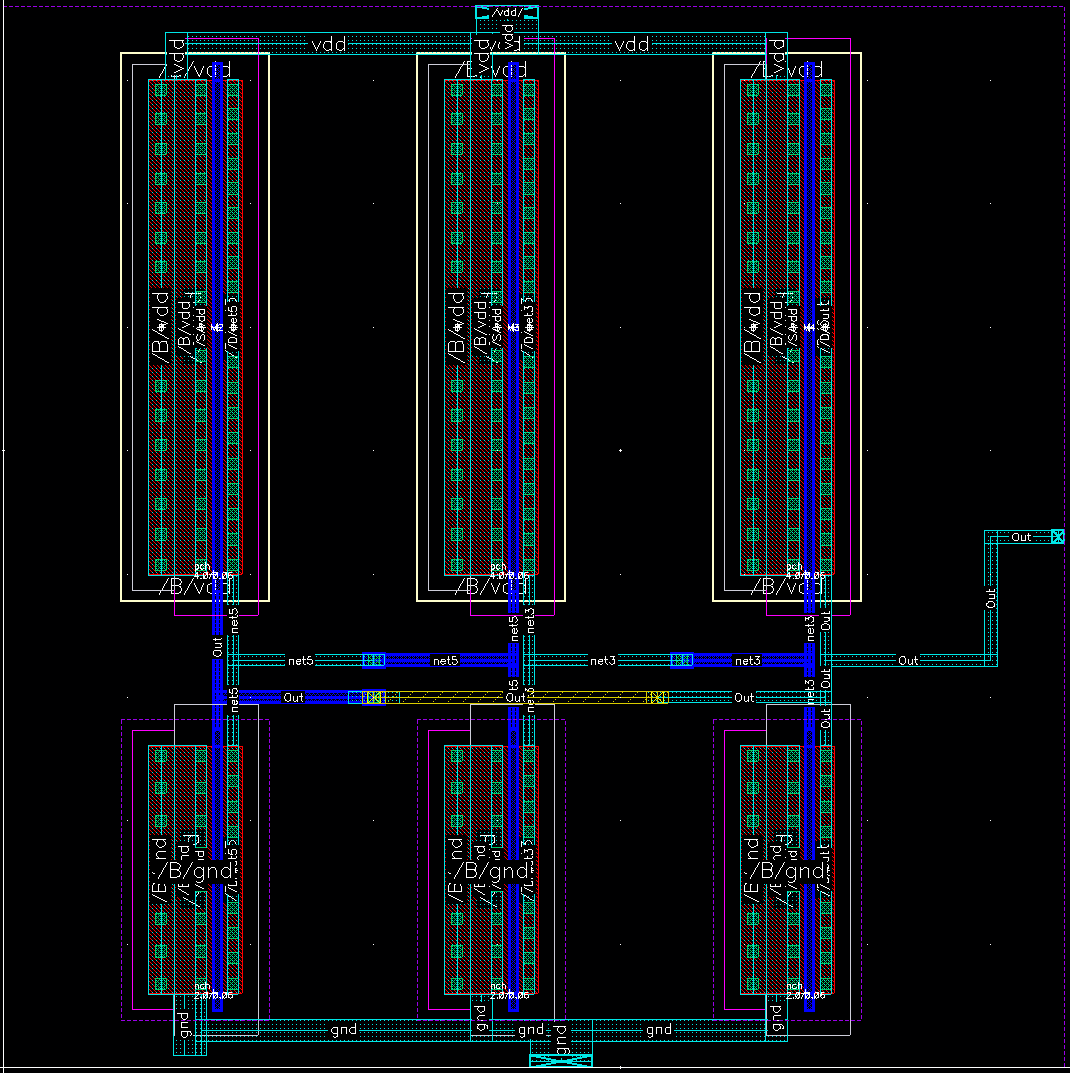
\includegraphics[width=0.38\textwidth]{layout.png}}
\caption{Manually routed layout core showing row-aligned PMOS and NMOS device matching ($8.6~\mu\text{m} \times 8.6~\mu\text{m}$).}
\label{fig:layout_core}
\end{figure}

\subsection{Matching and Mismatch Considerations}
Because the three delay cells nominally set identical stage delays, any
systematic difference between them translates directly into duty-cycle
distortion and phase error between the outputs. The layout was therefore
constrained so that the three stages are drawn as identical instances with
identical device orientation and poly pitch, and so that the interstage routing
is topologically the same for each cell rather than individually optimized.

The extracted per-net capacitances reported later in
Table~\ref{tab:parasitic_capacitance} indicate that this constraint was met: the
two purely internal nodes, \texttt{net3} and \texttt{net5}, differ by only
0.02~fF out of approximately 3.5~fF, i.e.\ below 1\%. The remaining asymmetry is
concentrated at the output node, which carries an additional 0.5~fF because it
also drives the external observation port. This is a deterministic,
layout-induced asymmetry rather than a random-mismatch effect.

Random $V_{\text{th}}$ and $\beta$ mismatch are not captured by the present
simulation-only flow. Dummy poly structures at the ends of the transistor rows,
continuous n-well and p-substrate guard rings, and matched dummy loading on the
internal nodes are identified as the measures required before tape-out, and are
noted as future work.

\subsection{Design Rule Checking}
After layout generation, Design Rule Checking (DRC) was performed to verify
compliance with the design rules of the 65-nm CMOS process. During the initial
verification stage, a Metal-1 spacing violation (rule M1.S.1, min
$0.09~\mu$m) was identified and corrected by adjusting the routing geometry.
After modification, the layout satisfied all essential DRC requirements. Some
remaining messages were associated with density-related rules and chip-level
layers (CSR and AP layers), which do not affect the functionality of the
oscillator core and are routinely addressed via automated dummy-fill insertion
during final mask assembly.

\subsection{Layout-Versus-Schematic Verification}
Layout-Versus-Schematic (LVS) verification was carried out to ensure consistency
between the physical layout and the original schematic. The comparison includes
device types, transistor dimensions, pin assignments, and net connectivity. The
extracted layout was found to be consistent with the schematic, indicating that
the designed topology was correctly transferred into the physical implementation.

Consequently, the effects observed in the post-layout simulations can be
attributed mainly to the parasitic elements introduced by interconnects and
device geometries rather than connectivity errors.

\section{Parasitic Extraction and Post-Layout Simulation Methodology}\label{sec:pex}

\subsection{RC Parasitic Extraction}
Following DRC and LVS verification, RC parasitic extraction was performed to
generate a Detailed Standard Parasitic Format (DSPF) netlist containing
distributed resistance and capacitance associated with interconnects and device
geometries~\cite{razavi_rf}. Compared with the schematic-level representation,
the extracted netlist provides a more realistic description of the oscillator
under practical operating conditions. The resulting per-net capacitances are
listed in Table~\ref{tab:parasitic_capacitance}.

\begin{table}[!b]
\caption{Extracted Per-Net Parasitic Capacitance from DSPF}
\label{tab:parasitic_capacitance}
\begin{center}
\begin{tabular}{cc}
\toprule
\textbf{Extracted Net Label} & \textbf{Parasitic Capacitance (fF)} \\
\midrule
\texttt{Out}  & 4.07 \\
\texttt{net3} & 3.54 \\
\texttt{net5} & 3.52 \\
\texttt{Vdd}  & 3.16 \\
\texttt{gnd}  & 3.01 \\
\bottomrule
\end{tabular}
\end{center}
\end{table}

The output node (\texttt{Out}) carries the largest capacitance because of the
feedback routing and external observation port, while the two internal nodes
are closely matched owing to the symmetrical layout arrangement. These
additional components increase the effective node loading and therefore the
propagation delay of each stage, so the oscillation frequency obtained from the
extracted netlist is lower than that predicted by the ideal schematic model.
The influence of these components is analyzed quantitatively in the following
section.

\subsection{Post-Layout Simulation Methodology}
Post-layout characterization used periodic steady-state (PSS) and periodic noise
(\texttt{pnoise}) analyses. Because the extracted DSPF netlist contains many
distributed RC elements, the simulation settings were tuned for stable
convergence and accurate steady-state solutions. The default \texttt{analogLib}
\texttt{port} primitive presents a $50~\Omega$ source/load resistance. Although
this matches standard test instruments, it overloads an unbuffered, low-power
sub-micron inverter stage, suppressing the loop gain below the Barkhausen
criterion and extinguishing the oscillation. A high-impedance
($1~\text{M}\Omega$) output port was therefore used to minimize core loading.
The PSS analysis ran in oscillator mode with sufficient stabilization time for
the amplitude and frequency to settle before the shooting algorithm was applied.
For phase noise,
\texttt{pnoise} was swept over offsets from 1~kHz to 100~MHz using the
time-average method with phase-modulation (PM) noise as the output. These
settings yielded stable simulations and reliable extraction of oscillation
frequency, power consumption, and phase-noise characteristics.

\subsection{Phase Noise and Figure-of-Merit Evaluation}
The phase-noise performance of the oscillator was evaluated from the
\texttt{pnoise} simulations~\cite{hajimiri_theory, razavi_phase}. Single-sideband
phase noise was measured at various offset frequencies relative to the carrier.
To facilitate comparison with previously reported oscillators, the figure of
merit (FoM) was calculated as~\cite{lee_tutorial}
\begin{equation}\label{eq:fom}
\text{FoM} = \mathcal{L}(\Delta f) - 20\log_{10}\!\left(\frac{f_0}{\Delta f}\right)
+ 10\log_{10}\!\left(\frac{P}{1~\text{mW}}\right)
\end{equation}
where $\mathcal{L}(\Delta f)$ is the single-sideband phase noise at an offset
frequency $\Delta f$, $f_0$ denotes the oscillation frequency, and $P$ represents
the power consumption.

\section{Results and Discussion}

\subsection{Post-Layout Transient Characteristics}
The post-layout transient response of the RC-extracted oscillator was
characterized under a 1.0-V supply. Fig.~\ref{fig:layout_sim_wave} shows stable
periodic oscillations with nearly rail-to-rail voltage swings ranging from
approximately $-0.05$~V to $1.04$~V.

\begin{figure}[!b]
\centering
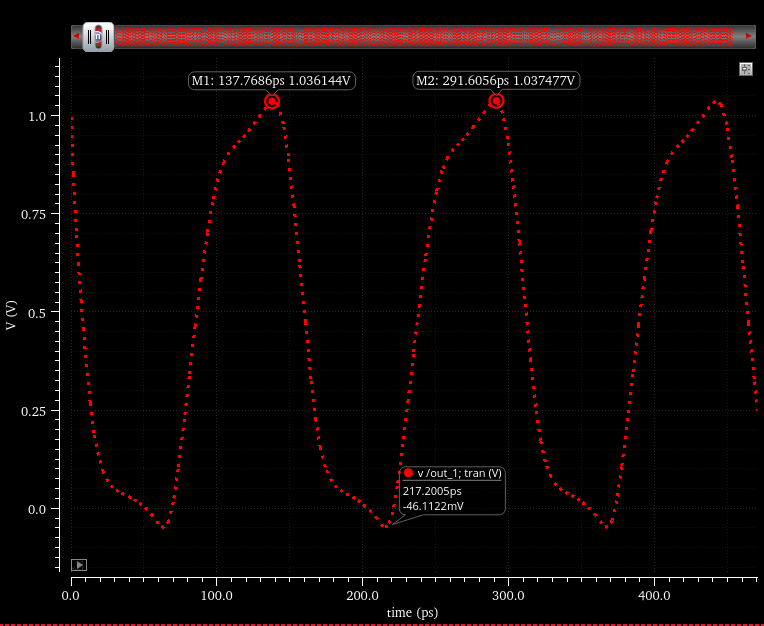
\includegraphics[width=0.45\textwidth]{layout_sim.png}
\caption{Post-layout (RC-extracted) transient output waveform showing stable rail-to-rail oscillation at 6.50~GHz with a period of 153.84~ps.}
\label{fig:layout_sim_wave}
\end{figure}

From the steady-state waveform, the oscillation period was measured as
\begin{equation}\label{eq:tpost}
T_{\text{post-layout}} = 153.84~\text{ps}
\end{equation}
which corresponds to an oscillation frequency of
\begin{equation}\label{eq:fpost}
f_{\text{osc,post-layout}} = \frac{1}{T_{\text{post-layout}}} = 6.50~\text{GHz}.
\end{equation}
The average supply current obtained from the transient simulation was
$286.3~\mu$A. Consequently, the power consumption of the oscillator is
\begin{equation}\label{eq:power}
P_{\text{dc}} = V_{\text{DD}} I_{\text{avg}} = 1.0~\text{V} \times 286.3~\mu\text{A} = 286.3~\mu\text{W}.
\end{equation}
Using \eqref{eq:period}, the average propagation delay of each inverter stage is
estimated to be
\begin{equation}\label{eq:tdpost}
t_{\text{d,post-layout}} = \frac{T_{\text{post-layout}}}{2N} = 25.6~\text{ps}.
\end{equation}

\subsection{Effect of Layout Parasitics}
Table~\ref{tab:pre_post} compares the pre-layout and post-layout performance. The
oscillation frequency decreases from 11.15~GHz to 6.50~GHz after parasitic
extraction, corresponding to a frequency reduction of approximately 41.7\%. In
addition, the average stage delay increases from 14.95~ps to 25.6~ps, a 71.2\%
increase. Because the transistor dimensions ($W/L$) and bias conditions remained
identical across both setups, this degradation is driven entirely by the
distributed RC parasitics embedded in the DSPF netlist.

\begin{table}[!t]
\caption{Pre-Layout Versus Post-Layout Performance}
\label{tab:pre_post}
\begin{center}
\begin{tabular}{lccc}
\toprule
\textbf{Parameter} & \textbf{Pre-Layout} & \textbf{Post-Layout} & \textbf{Change} \\
\midrule
Oscillation frequency & 11.15~GHz & 6.50~GHz  & $-41.7\%$ \\
Loop period           & 89.71~ps  & 153.84~ps & $+71.5\%$ \\
Stage delay $t_d$     & 14.95~ps  & 25.6~ps   & $+71.2\%$ \\
\bottomrule
\end{tabular}
\end{center}
\end{table}

\subsection{Phase Noise and Figure-of-Merit Performance}
Fig.~\ref{fig:pnoise_plot} shows the simulated phase-noise spectrum of the
oscillator. The curve exhibits a consistent $1/f^2$ slope across the offset
spectrum, confirming that white thermal-noise contributions dominate the
high-frequency phase-error profile~\cite{hajimiri_theory, razavi_phase}.

\begin{figure}[!b]
\centering
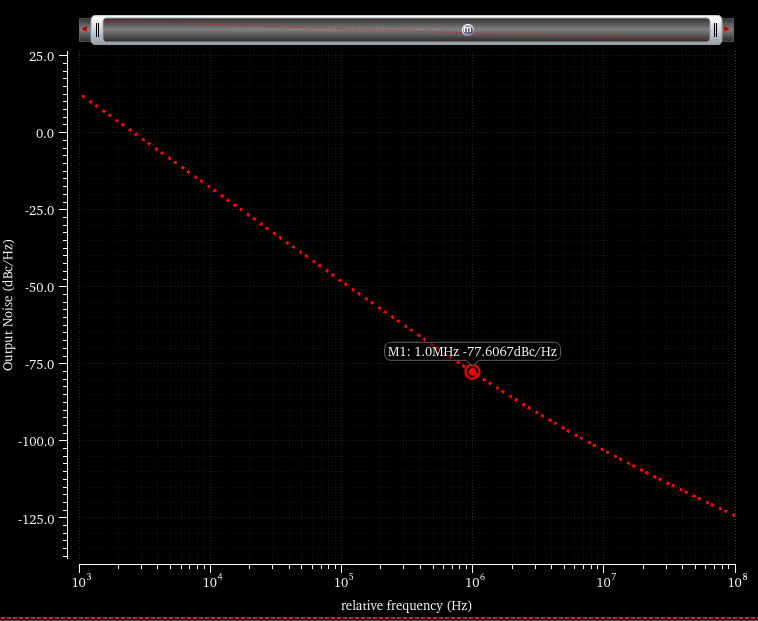
\includegraphics[width=0.45\textwidth]{pnoise.png}
\caption{Post-layout (RC-extracted) single-sideband phase noise versus relative offset frequency, showing $-77.6$~dBc/Hz at a 1~MHz offset.}
\label{fig:pnoise_plot}
\end{figure}

At an offset frequency of 1~MHz from the 6.50~GHz carrier, the single-sideband
phase noise is
\begin{equation}\label{eq:pn}
\mathcal{L}(1~\text{MHz}) = -77.6~\text{dBc/Hz}.
\end{equation}
At an offset frequency of 100~MHz, the phase noise decreases to $-124.3$~dBc/Hz.
Substituting the extracted post-layout metrics
($\mathcal{L}(1~\text{MHz}) = -77.6$~dBc/Hz, $f_0 = 6.50$~GHz, and
$P = 286.3~\mu$W) into \eqref{eq:fom} yields
\begin{align}\label{eq:fom_eval}
\text{FoM} &= -77.6 - 20\log_{10}\!\left(\frac{6.5\times 10^{9}}{1.0\times 10^{6}}\right)
+ 10\log_{10}\!\left(0.2863\right) \nonumber \\
&= -77.6 - 76.26 - 5.43 = -159.3~\text{dBc/Hz}.
\end{align}
The relatively low power consumption of $286.3~\mu$W contributes to the obtained
FoM value. Although the phase noise is typical of a conventional single-ended
ring oscillator, the results demonstrate that the proposed design achieves a
reasonable trade-off among oscillation frequency, power consumption, and spectral
purity.

\subsection{Comparison with Previous Works}
Table~\ref{tab:comparison} compares the proposed oscillator with representative
CMOS ring oscillators reported in the literature. As the design is characterized
by post-layout simulation, comparison with measured silicon should be treated
with caution. Even so, the proposed oscillator attains the best figure of merit
($-159.3$~dBc/Hz), surpassing the current-controlled RO in~\cite{nugroho_ring}
($-154.4$~dBc/Hz), the switched-capacitor VCO in~\cite{islam_mos}
($-155.5$~dBc/Hz), and the current-starved VCO in~\cite{anjum_csvco}
($-152.6$~dBc/Hz). It also uses the lowest supply (1.0~V), the most compact core
area ($73.96~\mu\text{m}^2$), and sub-milliwatt power ($286.3~\mu$W) on par
with the lowest-power designs. Other topologies, such as the quadrature design
in~\cite{pokharel_quadrature}, offer additional multiphase outputs at the cost
of more delay stages.

\begin{table}[!t]
\caption{Performance Comparison with Reported CMOS Ring Oscillators}
\label{tab:comparison}
\begin{center}
\footnotesize
\setlength{\tabcolsep}{3.5pt}
\renewcommand{\arraystretch}{1.15}
\begin{tabular}{lcccc}
\toprule
\textbf{Parameter} & \textbf{This} & \cite{nugroho_ring} & \cite{islam_mos} & \cite{anjum_csvco} \\
                   & \textbf{Work} & (2012) & (2017) & (2023) \\
\midrule
Technology        & 65~nm LP            & $0.18~\mu$m   & 90~nm      & 90~nm \\
Topology          & 3-st.\ RO           & 3-st.\ CCO    & SC-VCO     & CS-VCO \\
Verification      & Post-layout         & Simulation      & Schematic  & Sim. \\
Supply (V)        & 1.0                 & 1.8           & 1.8        & 1.8 \\
Freq.\ (GHz)      & 6.50                & 5.5           & 4.52--6.02 & 5.1 \\
Power             & $286.3~\mu$W        & $\leq 17.6$~mW & 0.295~mW  & $289~\mu$W \\
Phase noise\textsuperscript{a} & $-77.6$ & $-104$\textsuperscript{b} & N/R & $-74$ \\
\textbf{FoM (dBc/Hz)} & $\mathbf{-159.3}$ & $-154.4$  & $-155.5$   & $-152.6$ \\
Area ($\mu$m$^2$) & 73.96               & 300\textsuperscript{c} & N/R & N/R \\
\bottomrule
\end{tabular}
\end{center}
\footnotesize
\noindent RO: ring oscillator; CCO: current-controlled oscillator; SC-VCO: switched-capacitor ring VCO; CS-VCO: current-starved VCO; Sim.: schematic-level simulation; N/R: not reported. \textsuperscript{a}In dBc/Hz at 1~MHz offset unless noted. \textsuperscript{b}Reported at 4~MHz offset. \textsuperscript{c}Core area $0.0003$~mm$^2$.
\end{table}

Compared with previous studies, the main contribution of this work lies not in
introducing a new oscillator topology, nor in the extraction procedure itself,
which is a standard step in any modern design flow. It lies in reporting the
magnitude of the correction that this flow produces at a specific and fully
specified operating point. Had only the schematic-level result been reported, as
is common practice, this design would have appeared to operate 4.65~GHz above
what the extracted netlist supports. Table~\ref{tab:pre_post} makes that
correction explicit, and Table~\ref{tab:parasitic_capacitance} attributes it to
individual nets rather than to a single lumped factor.

\section{Conclusion}
This paper presented the physical implementation and parasitic-aware post-layout
characterization of a low-power three-stage ring oscillator in a 65-nm Low-Power
CMOS process. The flow followed here covers custom layout generation, physical
verification, RC parasitic extraction, and post-layout characterization using
periodic steady-state (PSS) and periodic noise (\texttt{pnoise}) analyses. Each
of these steps is well established; what is reported is the quantified effect
they reveal.

The extracted oscillator achieved a stable operating frequency of 6.50~GHz while
consuming only $286.3~\mu$W from a 1.0-V supply. The phase-noise performance was
characterized, resulting in a single-sideband phase noise of $-77.6$~dBc/Hz at a
1-MHz offset and a corresponding figure of merit of $-159.3$~dBc/Hz, occupying a
compact core area of $73.96~\mu\text{m}^2$.
The comparison between schematic-level and post-layout simulations demonstrates
the need to incorporate interconnect parasitics into the design flow. Overall,
the reported figures provide a concrete reference point for the parasitic budget
that must be anticipated when designing low-power, multi-gigahertz oscillator
blocks in advanced CMOS technologies. Against its own schematic baseline, the
design loses 41.7\% of its oscillation frequency and gains 71.2\% in stage
delay, driven by 3.5--4.1~fF of routing capacitance per internal node. Future
work will focus on experimental silicon validation, a systematic layout
optimization performed in two stages (device-core extraction compared against
the schematic, followed by interconnect analysis), the addition of explicit
frequency-tuning capability, and the application of low-noise delay-cell
techniques to further improve phase-noise performance.

\begin{thebibliography}{13}

\bibitem{maneatis_dll}
J.~G.~Maneatis, ``Low-jitter process-independent DLL and PLL based on self-biased techniques,'' \emph{IEEE J. Solid-State Circuits}, vol.~31, no.~11, pp.~1723--1732, Nov.~1996.

\bibitem{razavi_analog}
B.~Razavi, \emph{Design of Analog CMOS Integrated Circuits}. New York, NY, USA: McGraw-Hill, 2001.

\bibitem{lee_cmos}
T.~H.~Lee, \emph{The Design of CMOS Radio-Frequency Integrated Circuits}, 2nd~ed. Cambridge, U.K.: Cambridge Univ. Press, 2004.

\bibitem{maneatis_coupled}
J.~G.~Maneatis and M.~A.~Horowitz, ``Precise delay generation using coupled oscillators,'' \emph{IEEE J. Solid-State Circuits}, vol.~28, no.~12, pp.~1273--1282, Dec.~1993.

\bibitem{nugroho_ring}
P.~Nugroho, R.~K.~Pokharel, H.~Kanaya, and K.~Yoshida, ``A 5.9~GHz low power and wide tuning range CMOS current-controlled ring oscillator,'' \emph{Int. J. Elect. Comput. Eng.}, vol.~2, no.~3, pp.~293--300, Jun.~2012.

\bibitem{hajimiri_ring}
A.~Hajimiri, S.~Limotyrakis, and T.~H.~Lee, ``Jitter and phase noise in ring oscillators,'' \emph{IEEE J. Solid-State Circuits}, vol.~34, no.~6, pp.~790--804, Jun.~1999.

\bibitem{razavi_rf}
B.~Razavi, \emph{RF Microelectronics}, 2nd~ed. Upper Saddle River, NJ, USA: Prentice-Hall, 2012.

\bibitem{hajimiri_theory}
A.~Hajimiri and T.~H.~Lee, ``A general theory of phase noise in electrical oscillators,'' \emph{IEEE J. Solid-State Circuits}, vol.~33, no.~2, pp.~179--194, Feb.~1998.

\bibitem{razavi_phase}
B.~Razavi, ``A study of phase noise in CMOS oscillators,'' \emph{IEEE J. Solid-State Circuits}, vol.~31, no.~3, pp.~331--343, Mar.~1996.

\bibitem{lee_tutorial}
T.~H.~Lee and A.~Hajimiri, ``Oscillator phase noise: A tutorial,'' \emph{IEEE J. Solid-State Circuits}, vol.~35, no.~3, pp.~326--336, Mar.~2000.

\bibitem{islam_mos}
R. Islam, A. N. K. Suprotik, S. M. Z. Uddin, and M. T. Amin, ``Design and analysis of 3 stage ring oscillator based on MOS capacitance for wireless applications,'' in \emph{Proc. Int. Conf. Elect., Comput. Commun. Eng. (ECCE)}, Cox's Bazar, Bangladesh, Feb.~2017, pp.~723--727.

\bibitem{anjum_csvco}
N.~Anjum, V.~K.~S.~Yadav, and V.~Nath, ``Design and analysis of a low power current starved VCO for ISM band application,'' \emph{Int. J. Microsyst. IoT}, vol. 1, no. 2, pp. 82--98, 2023.

\bibitem{pokharel_quadrature}
R.~K.~Pokharel, S.~Lingala, A.~Anand, P.~Nugroho, A.~Tomar, H.~Kanaya, and K.~Yoshida, ``A wide tuning range CMOS quadrature ring oscillator with improved FoM for inductorless reconfigurable PLL,'' \emph{IEICE Trans. Electron.}, vol.~E94-C, no.~10, pp.~1524--1532, Oct.~2011.

\end{thebibliography}

\end{document}